\section{Theorie}
\label{sec:Theorie}

\subsection{Motivation und Zielsetzung}

Ziel dieses Versuches ist es, die Erzeugung eines Vakuums mithilfe von zwei
verschiedenen Pumpentypen zu verstehen und durchzuführen.
Durch Aufnahme einer Evakuierungskurve sowie einer Leckratenmessung können die
Hestellerangaben bezüglich des Saugvermögens der Pumpen überprüft werden.
Aufgrund des immer geringeren Atmosphärendrucks in großen Höhen ist die Vakuumphysik
in technischen Anwendungen von großer Bedeutung, um beispielweise Werkstoffe für
die Luft- und Raumfahrt zu entwickeln und zu testen.
Auch auf dem Boden müssen viele Prozesse im Vakuum stattfinden, um den störenden
Einfluss der Atmosphäre zu eliminieren. Ein Beispiel hierfür sind Teilchenbeschleuniger,
die ein sehr gutes Vakuum erforden, um Wechselwirkungen mit Gasteilchen zu verhindern.

\subsection{Theoretische Grundlagen}

Da ein perfektes Vakuum in der Praxis unmöglich zu erreichen ist, wird das Vakuum über verschiedene
Druckbereiche definiert. Erst ab Drücken von $p < \qty{300}{\milli\bar}$ wird der Begriff Vakuum verwendet,
da größere Drücke noch auf der Erdoberfläche anzutreffen sind.
In \autoref{tab:druecke} sind die verschiedenen Druckbereiche mit der dazugehörigen Definition des Vakuums
aufgeführt. In diesem Versuch wird maximal die Größenordnung eines Hochvakuums erreicht.
\begin{table}[H]
    \centering
    \caption{Druckbereiche in der Vakuumtechnik \cite{Pfeiffer_Vakuum}.}
    \label{tab:druecke}
    \begin{tabular}{c|c}
        \toprule
        Druckbereich & Druck / $\unit{\milli\bar}$\\
        \midrule
        Grobvakuum & $300 - 1$\\
        Feinvakuum & $1 - 10^{-3}$\\
        Hochvakuum & $10^{-3} - 10^{-8}$\\
        Ultrahochvakuum & $<10^{-8}$\\
        \bottomrule
    \end{tabular}
\end{table}
Die simpelste Beschreibung eines Gases liefert das Modell des idealen Gases. Hier werden alle Gasatome als punktförmig angenommen und
die Teilchen wechselwirken nicht untereinander. Es finden lediglich elastische Stößen untereinander und mit den Außenwänden statt.
Es gilt dann die Zustandsgleichung
\begin{equation}
    \label{eqn:gasgleichung}
    p V=N k_{\text{B}} T
\end{equation}
wobei $p$ für den Druck, $V$ für das Volumen, $N$ für die Teilchenzahl und $T$ für die Temperatur steht, $k_{\text{B}}$ ist die Boltzmann Konstante.
Bei konstanter Temperatur folgt sofort das Boyle-Mariott’schen Gesetz
\begin{equation}
    \label{eqn:bmgesetz}
    p V=const
\end{equation}
was einen antiproportionalen Zusammenhang zwischen $p$ und $V$ vorhersagt.
Die getroffenen Anahmen sind jedoch nicht für alle Komponenten der Atmosphäre anwendbar, zum Beispiel die stark polarisierten
Wassermoleküle im Wasserdampf wechselwirken stark miteinander, und die oben beschriebenen Zusammenhänge verlieren ihre Gültigkeit.
Um niedrige Drücke erreichen zu können, müssen derartige Verunreinigungen aus dem System entfernt werden.\\

Die gemeinsame Bewegung der Gasteilchen wird auch als \textit{Strömung} bezeichnet und hängt stark vom vorherrschenden Druck ab.
Je geringer der Druck, desto weniger Gasteilchen befinden sich im System und umso weniger Stöße finden untereinander statt.
Der durchschnittliche Weg, den ein Teilchen ohne Wechselwirkungen zurücklegen kann, wird als \textit{mittlere freie Weglänge} bezeichnet
und nimmt mit sinkendem Druck stark zu.
Ein Maß für die vorliegende Strömung ist die Knudsenzahl
\begin{equation}
    \notag
    K_{\text{n}} = \frac{\bar{l}}{d}
\end{equation}
bei der $\bar{l}$ für die mittlere freie Weglänge und $d$ für den Durchmesser des Rohres steht.
In \autoref{fig:stroemungen} sind die verschiedenen Arten von Strömungen in Abhängigkeit der Knudsenzahl
dargestellt.
\begin{figure}[H]
    \centering
    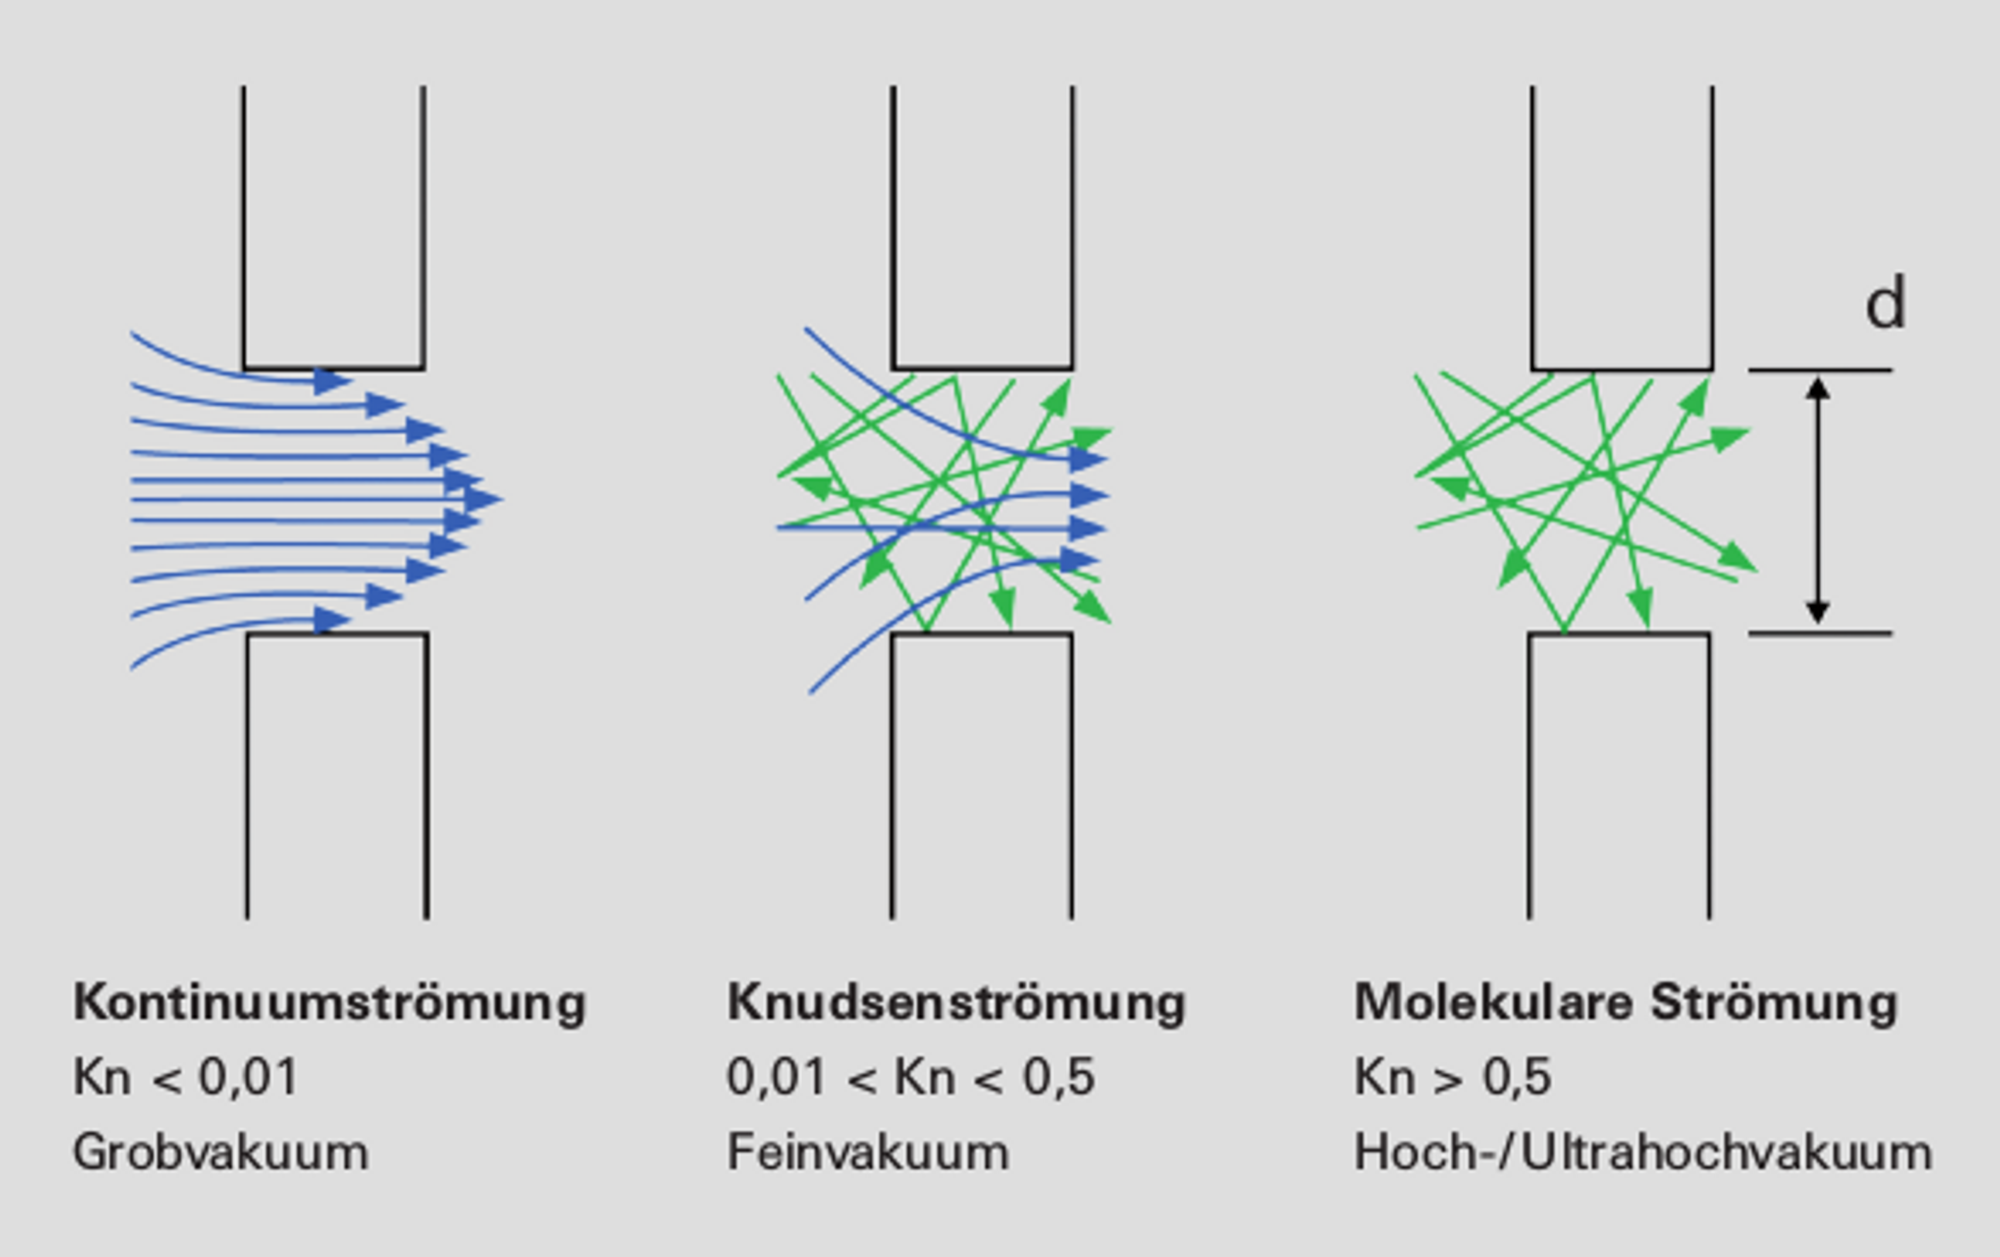
\includegraphics[width=0.6\textwidth]{content/pics/stroemung.png}
    \caption{Übersicht über die verschiedenen Strömungsarten \cite{Pfeiffer_Vakuum}.}
    \label{fig:stroemungen}
\end{figure}
Im Grobvakuum liegt laminare Strömung vor, die Gasteilchen bewegen sich also in zueinander parallelen Schichten.
Nimmt der Druck ab, so werden Wechselwirkungen zwischen den Teilchen immer seltener, bis schließlich nur noch
Stöße mit den Wänden stattfinden. Alle Teilchen bewegen sich unabhängig von einander und man nennt dies molekulare
Strömung.

\subsection{Vakuumerzeugung}

Um ein Vakuum zu erzeugen wird eine Pumpe benötigt, die das Gas gegen den Atmosphärendruck aus dem System pumpt.
Das Saugvermögen einer Pumpe ist über die Änderung des Volumens definiert:
\begin{equation}
    \label{eqn:saugvermoegen}
    S = \frac{\text{d}V}{\text{d}t}.
\end{equation}
Als Saugleistung bezeichnet man das Produkt aus Saugvermögen und Druck
\begin{equation}
    \label{eqn:saugleistung}
    q_{\text{pV}} = S \cdot P.
\end{equation}
In der Praxis wird die theoretische Saugleistung $S_0$ einer Pumpe nie ganz erreicht, da das sich zwangsläufig davorbefindende
Rohr einen Leitwert $L$ hat, der die Gasmenge begrenzt. Dieser kann analog zu einem reziproken elektrischen Widerstand verstanden werden.
Daher wird die effektive Saugleistung $S_{\text{eff}}$ verwendet, die sich gemäß
\begin{equation}
    \label{eqn:saugleistung_eff}
    \frac{1}{S_{\text{eff}}} = \frac{1}{S_{0}} + \frac{1}{L}
\end{equation}
berechnet. In der Regel ist das Saugvermögen einer Pumpe nicht konstant, sondern Abhängig vom Druck.
Nimmt man jedoch vereinfacht ein konstantes Saugvermögen an, so kann durch zeitliches Ableiten der Zustandsgleichung \eqref{eqn:gasgleichung}
die Differentialgleichung
\begin{equation}
    \notag
    \dot{p} \cdot V = -p \cdot S
\end{equation}
aufgestellt werden. Deren Lösung beschreibt die sogenannte Evakuierungskurve $p(t)$, die den zeitlichen Verlauf des Druckes gemäß
\begin{equation}
    \label{eqn:evakuierungskurve}
    p(t) = p_0 \cdot \exp{\left(-\frac{S}{V}\,t\right)}.
\end{equation}
beschreibt.
Ein System ist nie vollständig dicht, der Druckabfall durch verschiedene Lecks wird du die Leckrate
\begin{equation}
    \label{eqn:leckrate}
    Q = \frac{\symup{\Delta} p}{\symup{\Delta} t}\cdot V
\end{equation}
beschrieben, dabei steht $\symup{\Delta} p$ für den Druck, der in der Zeit $\symup{\Delta} t$ dazugekommen ist.
Über die Leckrate $Q$ lässt sich ebenfalls das zuvor beschriebene Saugvermögen $S$ berechnen mit der Formel
\begin{equation}
    \label{eqn:s_leck}
    S = \frac{Q}{p_{\text{G}}}.
\end{equation}
Dafür muss der Gleichgewichtsdruck $p_{\text{G}}$ bekannt sein. Bei diesem Druck gleicht sich die Saugleistung der Pumpe genau mit den
Undichtigkeiten der Lecks aus, sodass ein Gleichgewicht entsteht. In diesem Versuch werden zwei Typen von Vakuumpumpen verwendet:
\begin{enumerate}
    \item Drehschieberpumpe:
    \item Turbomolekularpumpe:
\end{enumerate}

\subsection{Vakuummessung}
